\chapter{Fejlesztői dokumentáció}
\label{ch:dev}

\section{Bevezetés}

Az alkalmazáshoz való technológiák kiválasztásakor fontos mind a felhasználó, mind a fejlesztő igényeit figyelmbe venni. Szerencsére, jelen esetben van megoldás, amely minden oldal számára a legtöbb kényelmet nyújtja, mégpedig a webalkalmazás. A felhasználó számára könnyű elérést, platformfüggetlenséget, és egy megszokott felületet hordoz magával, ami különösen fontos egy oktatási céllal rendelkező alkalmazásnál, hiszen még kevesebb akadályt helyez a felhasználó és a "tananyag" közé. Fejlesztői szempontból is kényelmes egy ilyen alkalmazást a böngészőre írni, hiszen a JavaScript ökoszisztémában könyvtárak és keretrendszerek tömkelege áll rendelkezésre, melyek segítségével gyorsan és hatékonyan lehet egy webalkalmazást fejleszteni.

\section{Adatforrás}

Az adatok a BKK\nomenclature{BKK}{Budapesti Közlekedési Központ} által szolgáltatott OpenData Portálon\cite{bkkopendata} nyilvánosan elérhető adatbázisból származnak. Az adatokat a BKK a GTFS\index{GTFS -- General Transit Feed Specification} (General Transit Feed Specification) formátumban teszik elérhetővé, ami egy Google-nél kifejlesztett\cite{gtfsabout} nyilvánosan elérhető specifikáció, mely egy szabványos formátumot definiál a tömegközlekedési adatok szolgáltatására.

\section{Tervezés és követelemények}

\subsection{Nem funkcionális követelmények}

\subsubsection{Termék követelmények}

\begin{enumerate}
    \item Hatékonyság
    \begin{compactitem}     
        \item A szoftver kezdeti megnyitásakor legkésőbb 5 másodperc alatt teljesen betöltődik és használhatóvá válik
        \item A szoftver általános használat közben folyatosan, megakadás közben fut egy középkategóriás számítógépen, egy modern böngészőben
        \begin{compactitem}     
            \item Kivétel ez alól az animált útvonaltervezés, amelynek a futása közben a szoftver akadozhat, de nem annyira, hogy használhatatlanná váljon, vagy megakadályozza az animáció leállítását
        \end{compactitem}
        \item A backend válaszideje API hívásokra nem több, mint 5 másodperc (bármilyen lehetséges, érvényes API hívásra)
        \item A szoftver felhasználói bevitelre adott válasz ideje nem több, mint 100 ezredmásodperc
        \begin{compactitem}     
            \item Ebbe beleértendő a betöltést jelző válasz, amíg az alkalmazás API hívásokra várakozik
        \end{compactitem}
        \item A szoftver nem használ a szükségesnél több processzorkapacitást (pl. nem használja processzortól függetlenül az összes elérhető teljesítményt)
    \end{compactitem}
    \item Megbízhatóság
    \begin{compactitem}
        \item A szoftverben ne legyen olyan egyszerűen előidézhető vagy gyakran bekövetkező hibajelenség, ami előfordulása esetén ellehetetleníti vagy jelentősen megnehezíti a szoftver használatát
    \end{compactitem}
    \item Biztonság
    \begin{compactitem}
        \item A szoftver ne tároljon felhasználói adatokat
        \item A szoftver ne tároljon érzékeny adatokat
        \item A szoftver ne tároljon jelszavakat
    \end{compactitem}
    \item Hordozhatóság
    \begin{compactitem}
        \item A szoftver kliens oldala bármilyen WebGL-t támogató modern böngészőben fut, különös tekintettel a Chromium alapú böngészőkre
        \item A szoftver a kliens oldalon állandó, stabil internetkapcsolatot és a szerverrel való kapcsolatatot igényel
        \item A szoftver szerver oldala az adatok letöltéséhez stabil internetkapcsolatot igényel, ezt követően csak a klienssel szükséges kommunikálnia
    \end{compactitem}
    \item Felhasználhatóság
    \begin{compactitem}
        \item A szoftver intuitív és könnyen használható
        \item A szoftver kliens oldalának a használatához nem szükséges külön telepítés, komoly számítógépes tapasztalattal nem rendelkező felhasználók számára is egyértelmű
        \item A weboldal felülete egy átlagos számítógéphasználó számára külső segítség nélkül elsajátítható, amennyiben ismerik a szoftver által bemutatott útkereső algoritmusokat
        \item A szoftver szerver oldalának az üzemeltetése hálózati és Docker-compose ismeretségeket igényel
    \end{compactitem}
\end{enumerate}

\subsubsection{Menedzselési követelemények}

\begin{enumerate}
    \item Környezeti
    \begin{compactitem}
        \item A szoftver kliens oldalon egy egeret és egy billentyűzetet igényel
        \item A szoftver szerver oldalának a futtatásához legalább egy középkategóriás számítógépnek megfelelő harver szükséges, eltekintve a perifériáktól
    \end{compactitem}
    \item Működési
    \begin{compactitem}
        \item A szoftver legfeljebb egy órás összefüggő időtartamokban lesz használva a kliens oldalon
        \item A szerver oldalon a szoftver folyamatosan fut, legfeljebb 4-5 naponta lehet szükséges karbantartási műveleteket végezni rajta, pl. a szoftver újraindítása (eltekintve az adatforrások frissítésétől)
    \end{compactitem}
    \item Fejlesztési
    \begin{compactitem}
        \item  Frontenden Node.js, React, TypeScript
        \begin{compactitem}
            \item  Térkép és adatok megjelenítéséhez deck.gl, react-map-gl
        \end{compactitem}
        \item  Backenden Node.js, Express, TypeScript
        \begin{compactitem}
            \item  REST API szerver
            \item  SQLite adatbázis
            \item  Adatok importálásához node-GTFS
        \end{compactitem}
        \item  Visual Studio Code fejlesztői környezet
        \item  Docker
        \item  64-bit architektúra
        \item  Verziókezeléshez Git kliens
    \end{compactitem}
    \item Fenntartási
    \begin{compactitem}
        \item Minden API végpont tesztelve és OpenAPI 3 formátumban dokumentálva van
    \end{compactitem}
\end{enumerate}

\subsubsection{Külső követelmények}

\begin{compactitem}
    \item A szoftverhez felhasznált külső forrásból származó médiafájlok jogtiszták
    \item A szoftver nem tartalmaz erkölcsileg megkérdőjelezhető, sértő tartalmat
\end{compactitem}

\subsection{Funkcionális követelmények}

\subsubsection{Funkciók}

\begin{enumerate}
    \item Útkeresés két megálló között budapesti tömegközlekedési járatokon
    \begin{itemize}
        \item Beállítások megadása
        \begin{itemize}
            \item Indulási és érkezési megálló kiválasztása
            \item Indulási idő megadása
            \item Útvonaltervezési algoritmus kiválasztása
            \begin{compactenum}
                \item BFS keresés
                \item Dijkstra algoritmus
                \item Mohó algoritmus
                \item A* algoritmus
            \end{compactenum}
            \item Útvonaltervezési algoritmus paramétereinek megadása
            \begin{compactitem}
                \item Maximális sétatávolság átszállások között
                \item A* algoritmus esetén: heurisztika súlyozása
            \end{compactitem}
        \end{itemize}
        \item Útvonaltervezés
        \begin{itemize}
            \item Algoritmus léptetése
            \item Algoritmus futtatásának indítása
            \item Algoritmus futtatásának szüneteltetése
            \item Algoritmus futtatásának folytatása
            \item Algoritmus visszaállítása alapállpotba
            \item Algoritmus eredményének megjelenítése
            \begin{compactitem}
                \item Potenciális útvonalak megjelenítése a térképen
                \item Soron következő megállók megjelenítése
            \end{compactitem}
        \end{itemize}
    \end{itemize}
\end{enumerate}

\subsection{Felhasználási eset diagram}

A program felhasználói eseteit a \ref{fig:use-case} ábra mutatja be.

\begin{figure}[H]
    \centering
    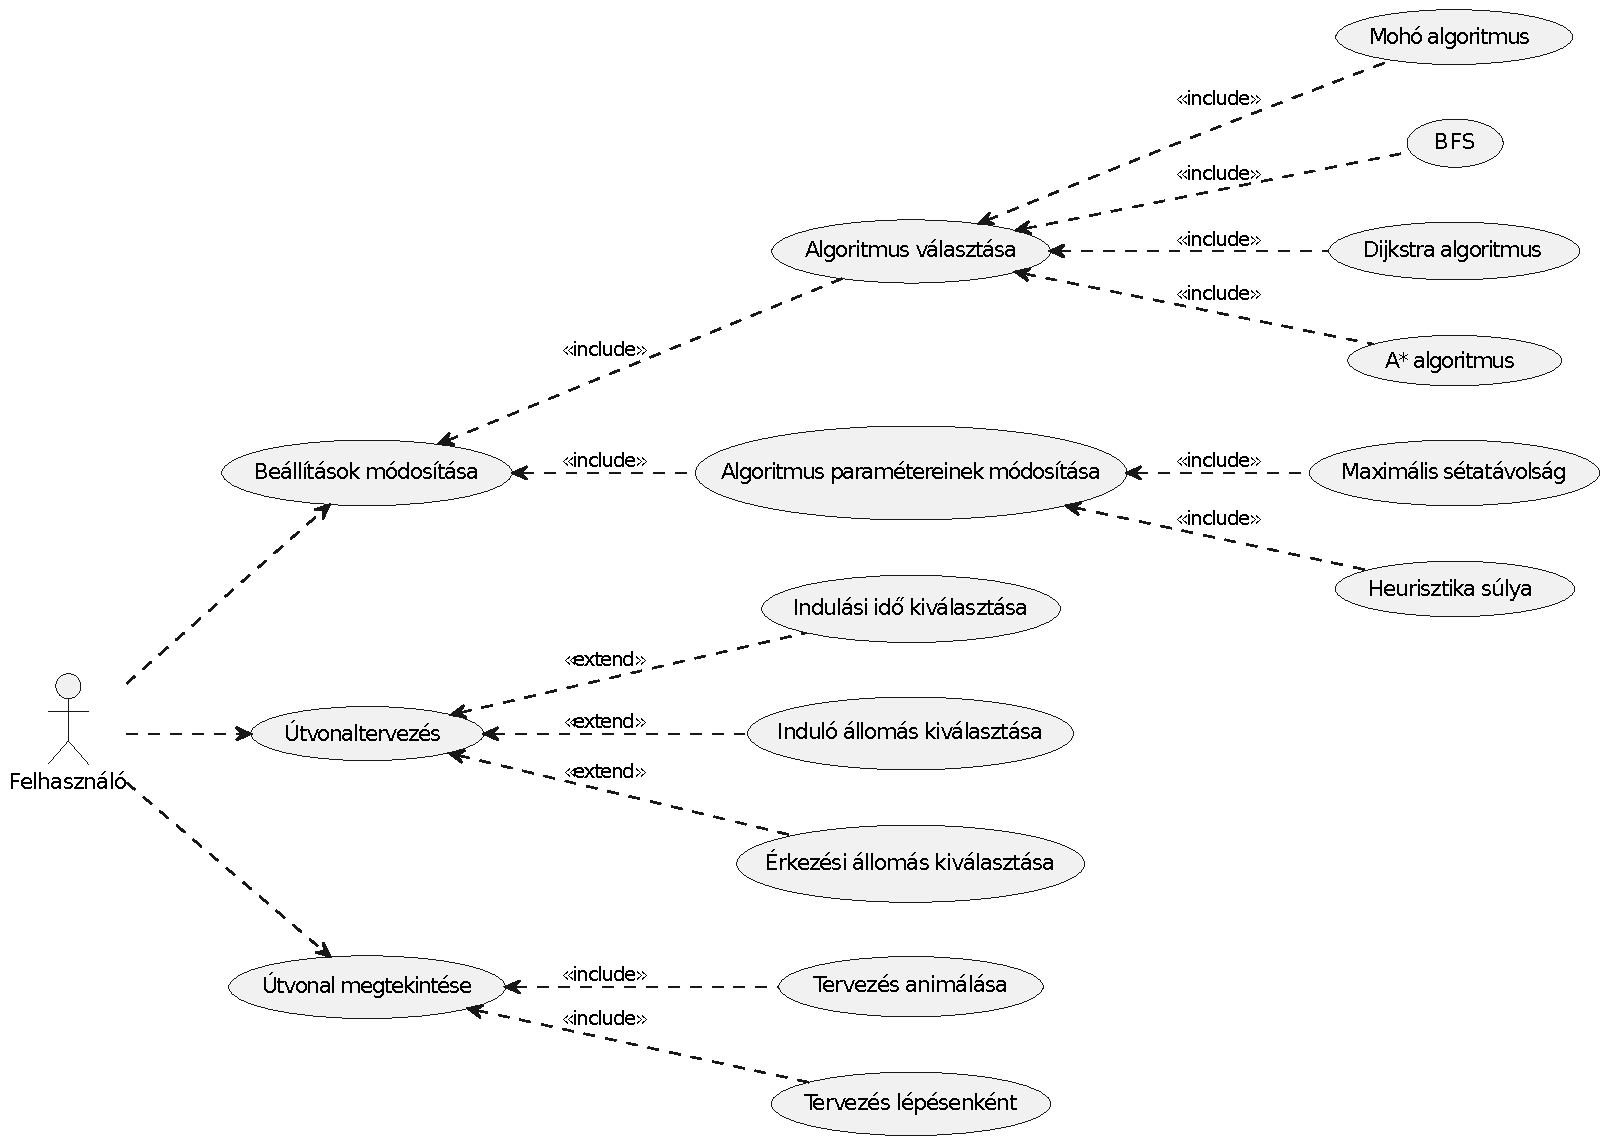
\includegraphics[width=1\textwidth]{use_case}
    \caption{Felhasználási eset diagram}
    \label{fig:use-case}
\end{figure}

\subsection{Felhasználói történet}

A felhasználói történetek a \ref{tab:user-stories-algorithm}., \ref{tab:user-stories-route}., \ref{tab:user-stories-parameters}., és a \ref{tab:user-stories-control}. táblákban olvashatóak.

\begin{table}[H]
    \centering
    \begin{tabular}{|c|c|p{10cm}|}
        \hline
        \textbf{1}  
        & AS A          & Felhasználó \\ \hline
        & I WANT TO     & Megváltoztatni a használt algoritmust \\ \hline
        & SO THAT       & Más algoritmusok vizualizációját tekintsem meg \\ \hline
        \hline
        1 & GIVEN   & A "beállítások" fül van kiválasztva \\ \hline
        & WHEN    & A legördülő menüben a \textbf{BFS algoritmust} választom \\ \hline
        & THEN    & Az útvonaltervezés a \textbf{BFS algoritmussal} fog történni \\ \hline
        \hline
        2 & GIVEN   & A "beállítások" fül van kiválasztva \\ \hline
        & WHEN    & A legördülő menüben a \textbf{Mohó algoritmust} választom \\ \hline
        & THEN    & Az útvonaltervezés a \textbf{Mohó algoritmussal} fog történni \\ \hline
        \hline
        3 & GIVEN   & A "beállítások" fül van kiválasztva \\ \hline
        & WHEN    & A legördülő menüben az \textbf{A* algoritmust} választom \\ \hline
        & THEN    & Az útvonaltervezés \textbf{A* algoritmussal} fog történni \\ \hline
        \hline
        4 & GIVEN   & A "beállítások" fül van kiválasztva \\ \hline
        & WHEN    & A legördülő menüben a \textbf{Dijkstra algoritmust} választom \\ \hline
        & THEN    & Az útvonaltervezés a \textbf{Dijkstra algoritmussal} fog történni \\ \hline
    \end{tabular}
    \caption{Felhasználói történet: algoritmus választása}
    \label{tab:user-stories-algorithm}
\end{table}

\begin{table}[H]
    \centering
    \begin{tabular}{|c|c|p{10cm}|}
    \hline
    \textbf{2}
    & AS A          & Felhasználó \\ \hline
    & I WANT TO     & Kiválasztani az tervezendő útvonalat \\ \hline
    & SO THAT       & Megtekinthetem az útvonaltervezést a választott útvonalon \\ \hline
    \hline
    1 & GIVEN   & A "beállítások" fül van kiválasztva \\ \hline
    & WHEN    & Az "indulási állomás" mezőbe beírom egy állomás nevét \\ \hline
    & THEN    & Az útvonaltervezés a kiválasztott állomástól fog indulni \\ \hline
    \hline
    2 & GIVEN   & A "beállítások" fül van kiválasztva \\ \hline
    & WHEN    & Az "érkezési állomás" mezőbe beírom egy állomás nevét \\ \hline
    & THEN    & Az útvonaltervezés a kiválasztott állomást fogja megkeresni \\ \hline
    \hline
    3 & GIVEN   & A "beállítások" fül van kiválasztva \\ \hline
    & WHEN    & Az "indulási idő" mezőben kiválasztok egy időt \\ \hline
    & THEN    & Az útvonal első járata a kiválasztott idő után fog indulni \\ \hline
    \end{tabular}
    \caption{Felhasználói történet: útvonal kiválasztása}
    \label{tab:user-stories-route}
\end{table}

\begin{table}[H]
    \centering
    \begin{tabular}{|c|c|p{10cm}|}
        \hline
        \textbf{3}
        & AS A          & Felhasználó \\ \hline
        & I WANT TO     & Megváltoztatni a használt algoritmus paramétereit \\ \hline
        & SO THAT       & Más paraméterekkel tekintsem meg az útvonaltervezést \\ \hline
        \hline
        1 & GIVEN & A "beállítások" fül van kiválasztva \\ \hline
        & AND     & Az A* algoritmus van kiválasztva \\ \hline
        & WHEN    & A "heuristika súlya" mezőben módosítom a súlyt \\ \hline
        & THEN    & Az útvonaltervezés a választott súlyt fogja használni \\ \hline
        \hline
        2 & GIVEN & A "beállítások" fül van kiválasztva \\ \hline
        & WHEN    & A "gyalogos távolság" mezőben módosítom a távolságot \\ \hline
        & THEN    & Az algoritmus által tervezett útvonal részeként nem fog szerepelni
                    két járat között olyan átszállás, ami a megadottnál nagyobb távolságú \\ \hline
    \end{tabular}
    \caption{Felhasználói történet: algoritmus paramétereinek módosítása}
    \label{tab:user-stories-parameters}
\end{table}

\begin{table}[H]
    \centering
    \begin{tabular}{|c|c|p{10cm}|}
        \hline
        \textbf{4}
        & AS A          & Felhasználó \\ \hline
        & I WANT TO     & Interaktívan megtekinteni a tervezett útvonalat \\ \hline
        & SO THAT       & Láthatom az útvonaltervezés lépéseit \\ \hline
        \hline
        1 & GIVEN   & Az "útvonal" fül van kiválasztva \\ \hline
        & AND     & Válaszottam indulási állomást, érkezési állomást és indulási időt \\ \hline
        & AND     & Az algoritmus még nem talált utat a kiválasztott állomások között \\ \hline
        & WHEN    & A "következő lépés" gombra kattintok \\ \hline
        & THEN    & Az algoritmus elvégzi a következő lépését \\ \hline
        \hline
        2 & GIVEN   & Az "útvonal" fül van kiválasztva \\ \hline
        & AND     & Válaszottam indulási állomást, érkezési állomást és indulási időt \\ \hline
        & AND     & Az algoritmus még nem talált utat a kiválasztott állomások között \\ \hline
        & WHEN    & Az "animáció indítása" gombra kattintok \\ \hline
        & THEN    & Az algoritmus addig fut, amíg nem találja meg a cél állomást, vagy nem szüneteltetem \\ \hline
        \hline
        3 & GIVEN   & Az "útvonal" fül van kiválasztva \\ \hline
        & AND     & Az algoritmus az "animáció indítása" gombra való kattintás hatására fut \\ \hline
        & WHEN    & Az "animáció szüneteltetése" gombra kattintok \\ \hline
        & THEN    & A program további interakció nélkül nem végez több lépést \\ \hline
        \hline
        4 & GIVEN   & Az "útvonal" fül van kiválasztva \\ \hline
        & AND     & Az algoritmus talált utat a kiválasztott állomások között \\ \hline
        & WHEN    & A "visszaállítás" gombra kattintok \\ \hline
        & THEN    & Az algoritmus "elfelejti" a talált utat és megállókat, és az alapállapotába áll \\ \hline
    \end{tabular}
    \caption{Felhasználói történetek}
    \label{tab:user-stories-control}
\end{table}

\subsection{Felhasználói felület tervek}

Az alkalmazás nyitóoldala a \ref{fig:wireframe-settings}. ábrán látható.

\begin{figure}[H]
    \centering
    
\includegraphics[width=1\textwidth]{wireframe_settings}
    \caption{Beállítások felület terve}
    \label{fig:wireframe-settings}
\end{figure}

Innen az "indulási állomás" és az "érkezési állomás" mezőkbe beírva egy állomás nevének a részletét rákereshetünk arra, és kiválaszthatjuk azt. A keresési találatok megjelenítését a \ref{fig:wireframe-search}. ábra mutatja be.

\begin{figure}[H]
    \centering
    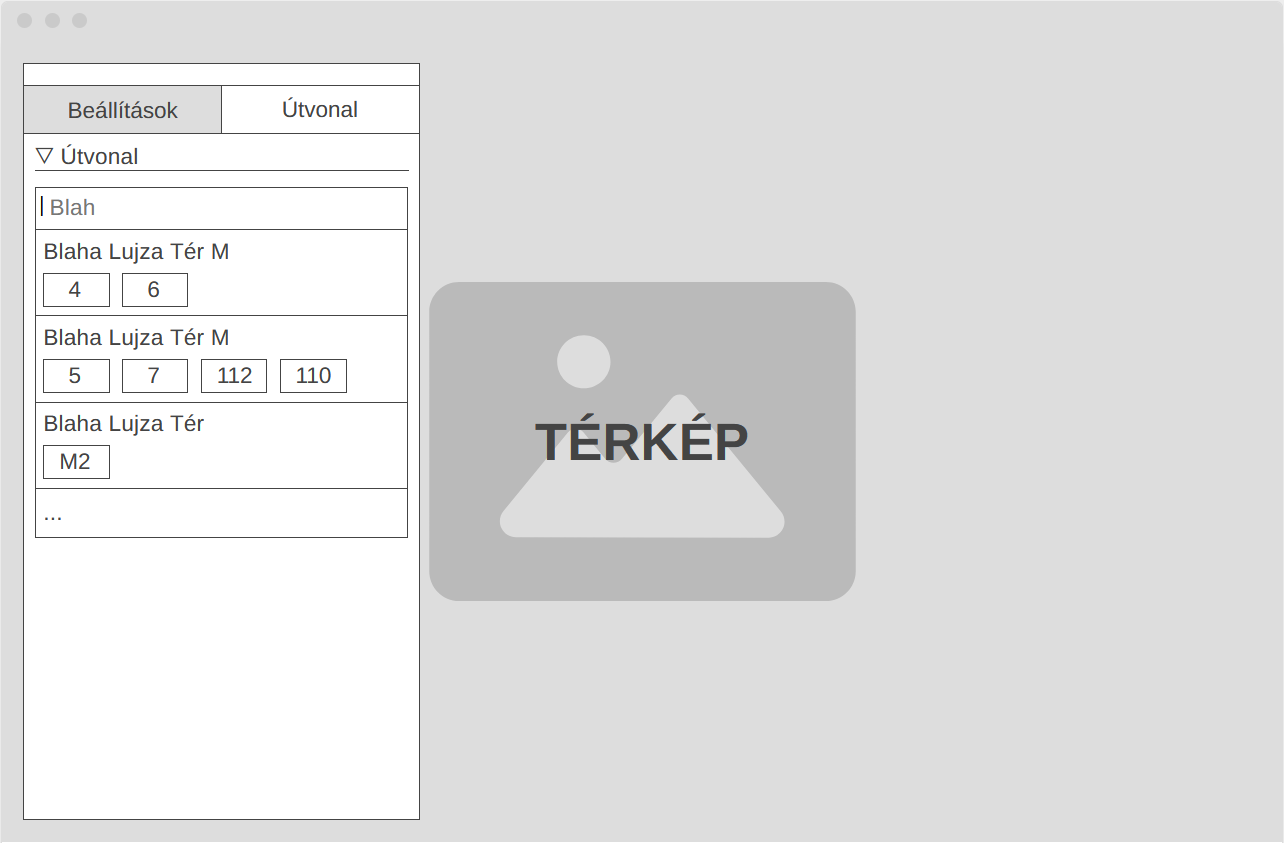
\includegraphics[width=1\textwidth]{wireframe_search}
    \caption{Megálló keresésének felület terve}
    \label{fig:wireframe-search}
\end{figure}

Ezen állomások kiválasztása után az "indulási idő" mezőben kiválaszthatjuk az indulási időt (vagy az alapértelmezettet használhatjuk), majd az "útvonal" gombra kattintva a \ref{fig:wireframe-plan}. ábrán látható felületen irányíthatjuk az algoritmus futását, és tekinthetjük meg annak állapotát és eredményét.

\begin{figure}[H]
    \centering
    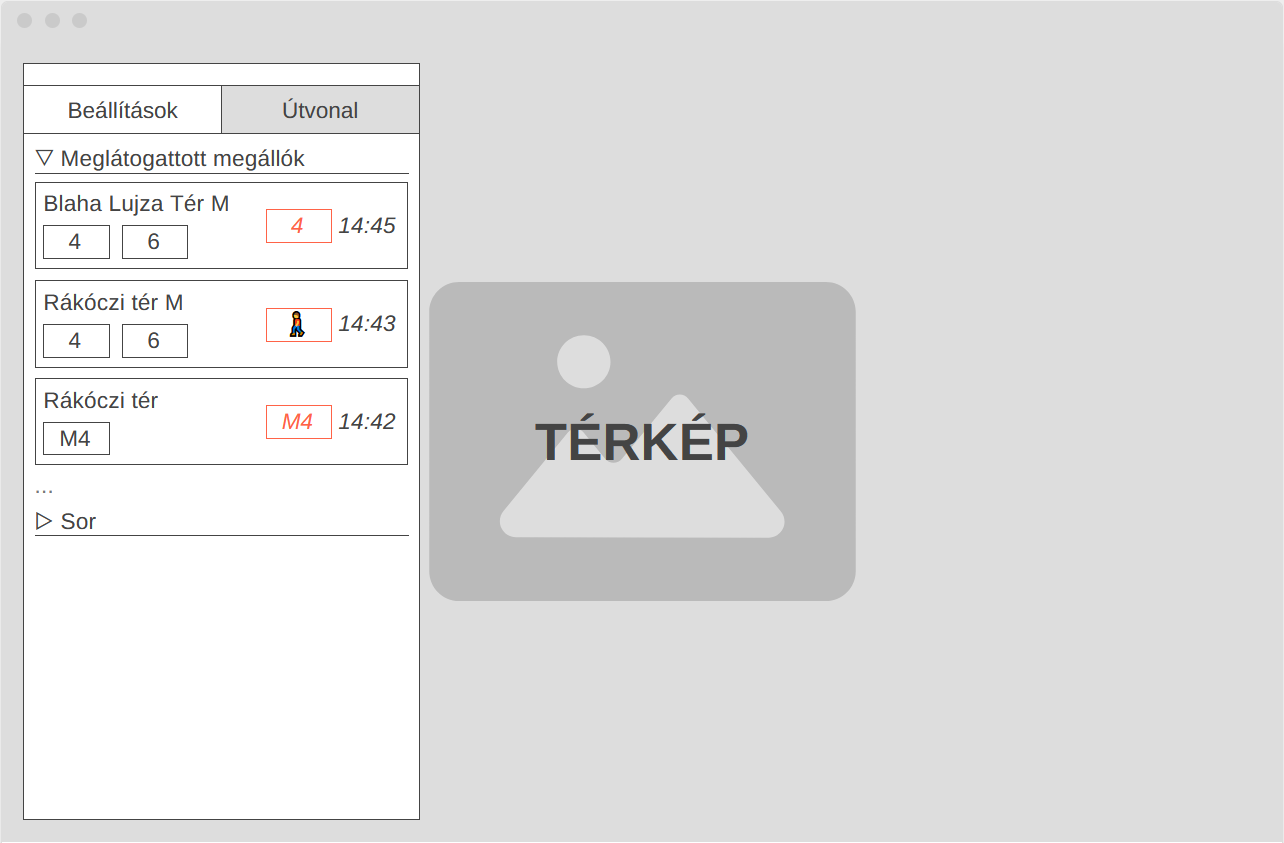
\includegraphics[width=1\textwidth]{wireframe_plan}
    \caption{Algoritmus irányításának felület terve}
    \label{fig:wireframe-plan}
\end{figure}

\section{Magas szintű áttekintés}

\subsection{Alkalmazás felépítése}

Az alkalmazás egy backendből és egy frontendből áll, REST API-n\nomenclature{REST}{REpresentational State Transfer, egy szoftverarchitektúra típus, ami megkötésekkel garantálja többek között az adatok gyorsítótárazhatóságát\cite{rest}} keresztül kommunikálnak egymással. A backend feladata a GTFS formátumban elérhető adatok adatbázisba való betöltése, valamit ezen adatok szolgáltatása a frontend számára. A frontend egy webalkalmazás, mely a felhasználói felületet biztosítja a felhasználók számára.

Fontos megemlíteni, hogy az útvonal tervezése és az algoritmusok futtatása a frontenden történik. Azért választottam ezt a megoldást, hogy az API-n átvitt adatok komplexitását minimalizáljam; mivel a frontendnek egyébként is szüksége van az összes információra az algoritmus belső állapotáról, így a számításokat a frontendre helyezve elég az adatbázis-lekérdezéseket és azok eredményét kommunikálni a kettő között.

\subsection{Verziókövetés}

A változtatásokat \textit{git} használatával tartom számon, így a fejlesztés során bármikor visszaállítható egy korábbi verzió, vagy összehasonlítható két verzió közötti különbség.

\subsection{Backend áttekintés}

% \footnote{A \textit{Node.js} egy platform, ami JavaScript kód szerveroldali futtatását teszi lehetővé}
A backend egy \textit{Node.js} alapú alkalmazás, mely az \textit{Express.js} keretrendszert használja a REST API megvalósítására. Fontos tényező volt a környezet kiválasztásában, hogy az NPM\footnote{Az NPM egy csomagnyilvántartás JavaScript csomagoknak, saját állításuk szerint a világ legnagyobb csomagnyilvántartása\cite{nodeabout}}-en megtalálható \textit{node-gtfs}\cite{nodegtfs} csomag egyike volt a kevés elérhető könyvtáraknak\footnote{A GTFS adatok feldolgozására való könyvtárak listája megtalálható a \url{https://gtfs.org/resources/gtfs/} oldalon \textit(Letöltés dátuma: 2024.11.22.)}, amelyek képesek GTFS adatok adatbázisba való betöltésére és lekérdezésére. További előnye a \textit{Node.js} backend választásának, hogy a frontenddel azonos a fejlesztői környezet, így a fejlesztéshez nem kell új programokat telepíteni, és a frontend és a backend fejlesztése közötti váltást is egyszerűvé teszi.

Hogy a backend akár távoli szerveren is egyszerűen beindítható legyen a teljes tesztkörnyezet reprodukálása nélkül, az alkalmazást Dockerizáljuk\index{Docker -- virtualizációs technológia, mely alkalmazások platformfüggetlen futtatását teszi lehetővé}; így egy \texttt{git clone [repo] \&\& docker compose up -d} paranccsal bárhol egyszerűen futtatható a backend (ahol a Docker és a git telepítve van).

Az olvashatóság és karbantarthatóság érdekében a backend kódja TypeScript\footnote{A TypeScript egy nyelv, ami a JavaScriptre épül, de statikus típusokat is támogat\cite{typescript}} nyelven íródik.

\subsection{Frontend áttekintés}

A frontend egy \textit{React} webalkalmazás, mely a backendhez hasonlóan \textit{TypeScript} nyelven van írva. A \textit{React} egy komponens alapú könyvtár, melynek segítségével a felhasználói felületet kisebb, önállóan működő komponensekre bonthatjuk, így a kód olvashatóbb és karbantarthatóbb lesz. Azért erre esett a választásom Angular és Vue helyett, mert a React népszerűsége messze túlszárnyalja ezekét\cite{reactcomparison}, így a fejlesztők számára könnyen elérhetőek a segédanyagok és a közösség támogatása is.

Az utak térképen való megjelenítéséhez a két fő lehetőség a \textit{deck.gl}, és az erre épülő\cite{kepler} \textit{kepler.gl}, amit az Ubernél fejlesztettek nagy volumenű utazási adat megjelenítésére. A döntésem a \textit{deck.gl}-re esett, mert egyszerű utak és megállók megjelenítésére szükségtelen a \textit{kepler.gl} komplexitása, illetve a \textit{deck.gl} dokumentációját is részletesebbnek és könnyebben érthetőnek találtam. A React választása melletti érv volt az is, hogy a \textit{deck.gl} a Reacthoz biztosít előre elkészített komponenseket (más könyvtárakkal ellentétben), így a két technológia jól egymásra épül.

\subsection{Fejlesztői környezet felállítása}

Az alkalmazás fejlesztéséhez a következő programok telepítése szükséges:

\begin{compactitem}
    \item \textit{Node.js (és npm csomagkezelő)}: Bár a backend és a frontend is Dockerben futtatható, az Intellisense számára érdemes a host gépen is telepíteni a használt csomagokat.
    \item \textit{Docker}
    \item \textit{git}
    \item \textit{IDE/szövegszerkesztő}: Én a Visual Studio Code-ot használom és javaslom, mert ingyenes és egyszerűen bővíthető JavaScript és Docker támogatáshoz, de használható más IDE (pl. WebStorm) is.
\end{compactitem}

Függőségek telepítéséhez a backend és a frontend mappákban a \texttt{npm install} parancsot kell futtatni.

\subsection{Alkalmazás futtatása}

Az alkalmazást fejlesztéshez is Dockerben futtatjuk, hogy a program írásakor feltételezhessük, hogy mindig ugyanaz a környezet áll rendelkezésre. A Dockerfile a frontend és a backend esetében egyaránt négy stage-et tartalmaz:

\begin{compactenum}
    \item \texttt{base}: Az alap image, amely `node:lts-alpine`-t használ. Erre épül az összes többi stage.
    \item \texttt{development}: Az \texttt{npm run dev} parancsot futtatja. Ennek a futtatásakor az alkalmazás figyeli a fájlrendszert\footnote{A fájlrendszer figyeléséről frontend esetén a \textit{vite}, backend esetén a \textit{tsx} gondoskodik.}, és újraindítja a kódot minden alkalommal, amikor egy fájl frissül (frontenden csak azokat a komponeneseket, amiket érinti a frissítés --- ezt HMR-nek, azaz Hot Module Reload-nak hívják).
    \item \texttt{build}: Az \texttt{npm run build} parancsot futtatja, ami JavaScript-re fordítja a TypeScript kódot.
    \item \texttt{production}: A \texttt{build}-ből lemásolja a lefordított kódot és futtatja azt.
\end{compactenum}

A stage-ek külön bontásának köszönhetően a \texttt{production} image a lehető legkisebb lesz, és a Docker építéskor gyorsítótárban tudja tárolni a lépések közös elemeit. A különválasztott fejlesztői és a produkciós környezetnek megfelelően két külön Docker Compose fájl is található a projektben: a \texttt{docker-compose.debug.yml} a fejlesztői környezetet állítja fel, míg a \texttt{docker-compose.yml} a produkciós környezetet. Az indításkor az ennek megfelelő parancs használandó (\ref{src:compose-dev}).

\lstset{caption={Alkalmazás indítása különböző konfigurációkban}, label=src:compose-dev}
\begin{lstlisting}[language={bash}]
    # Fejlesztői környezet indítása
    docker compose -f docker-compose.debug.yml up -d --build

    # Produkciós környezet indítása
    docker compose up -d --build
\end{lstlisting}

Bár produkciós környezethez minden adott, hogy Dockerből futtatható legyen az alkalmazás mindkét része, a frontend statikusan kiszolgálható fájlokra fordul le, így ezt nem érdemes egy Docker konténerben futtatni. Ehelyett javasolt az \texttt{npm run build} által a \textit{dist} könyvtárba lefordított fájlokat egy webszerveren keresztül kiszolgálni, például Nginx vagy Apache HTTP szerver segítségével.

\section{Backend}

\subsection{Könyvtárszerkezet}

A backend könyvtárszerkezete a következő:

\begin{compactitem}
    \item \texttt{src}: A forráskódokat tartalmazó könyvtár.
    \item \texttt{src/configs}: Konfigurációs fájlok helye.
    \item \texttt{src/models}: Adatbázis sémák helye.
    \item \texttt{src/routes}: A REST API végpontokat tartalmazó fájlok.
    \item \texttt{src/utils}: Segédfüggvények adatok betöltésére és lekérdezésére.
    \item \texttt{src/index.ts}: Az alkalmazás belépési pontja.
    \item \texttt{.dockerignore}: \texttt{.gitignore}-hoz hasonlóan a Docker által figyelmen kívül hagyott fájlok listája.
    \item \texttt{Dockerfile}: A Docker image felépítéséhez szükséges fájl.
    \item \texttt{drizzle.config.ts}: A \textit{drizzle-kit} konfigurációs fájlja (részletek a \ref{TODO} fejezetben).
    \item \texttt{package.json}: A függőségeket és egyéb metainformációkat tartalmazó fájl.
    \item \texttt{package-lock.json}: Az \texttt{npm} csomagkezelő által generált fájl, mely a telepített függőségek pontos verzióit tartalmazza.
    \item \texttt{generate-types.ts}: Segédscript, mely az adatbázis sémából TypeScript típusokat generál a frontend számára.
    \item \texttt{tsconfig.json}: A TypeScript konfigurációs fájl.
\end{compactitem}

\subsection{Adatbázis}

A program indításakor az első lépés az adatbázis létrehozása és feltöltése a GTFS adatokkal. Az adatok betöltésére és lekérdezésére a korábban említett \textit{node-gtfs} csomagot használom. (NPM-en és kódban egyszerűen \textit{gtfs}-nek hívják, korábban a GitHub-on szereplő nevét használtam a szabványtól való megkülönböztetés végett. A továbbiakban kisbetűvel írva, gtfs-ként fogok hivatkozni rá.)

A gtfs a GTFS adatokat egy SQLite adatbázisba tölti be, melynek sémája a GTFS specifikációban meghatározott táblákat tartalmazza (\ref{fig:gtfs-schema}). 

\pagebreak

\begin{figure}[H]
    \centering
    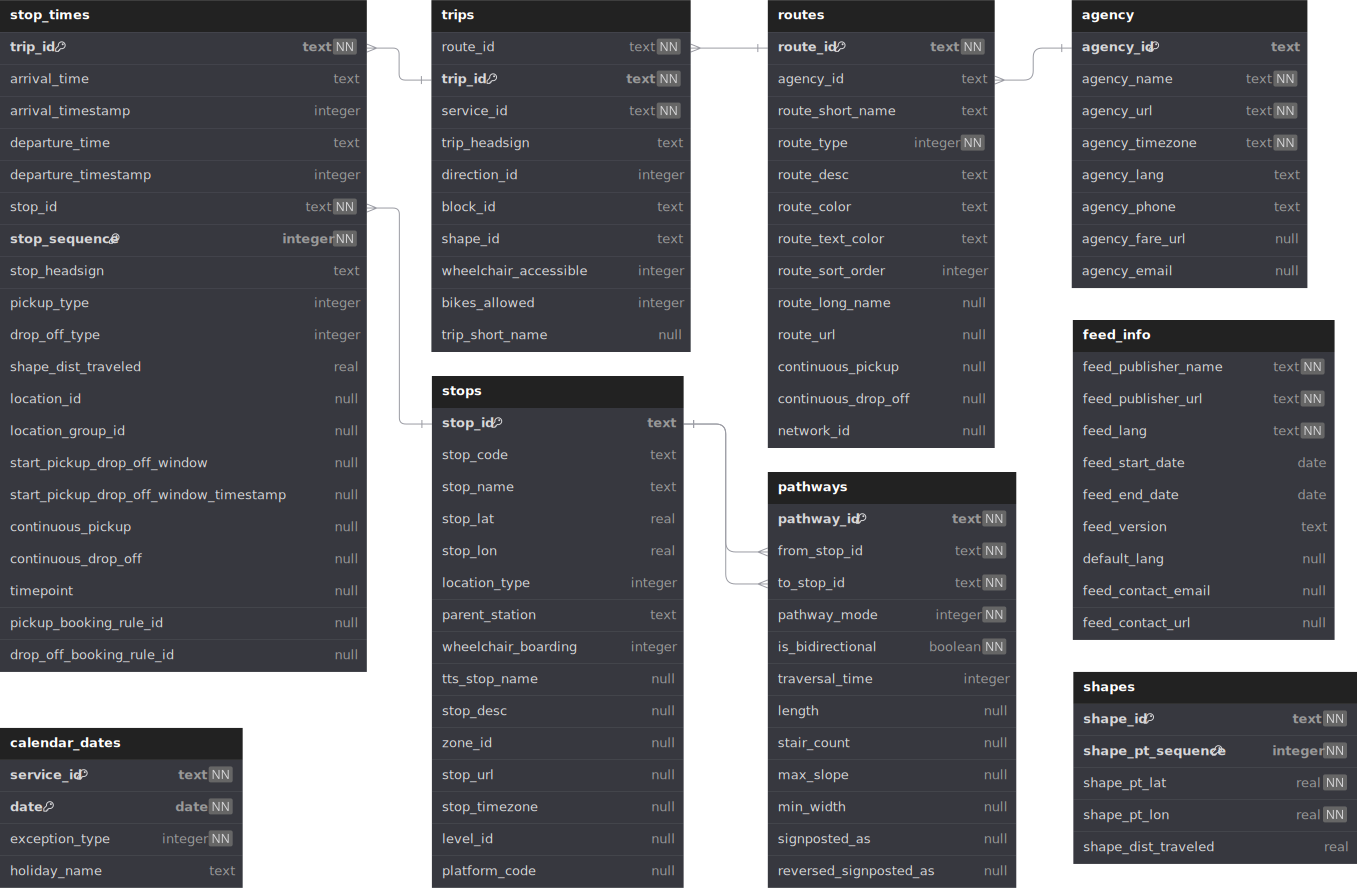
\includegraphics[width=1\textwidth]{entity_relationship}
    \caption{GTFS adatbázis sémája}
    \label{fig:gtfs-schema}
\end{figure}

\pagebreak

\textit{Megjegyzés: A teljes GTFS szabvány ennél jóval több táblát tartalmaz, de a legtöbbjük opcionális. A \ref{fig:gtfs-schema} ábra csak azokat a táblákat tartalmazza, amelyeket a BKK OpenData Portálán elérhető adatok tartalmaznak. Ezen táblákban is vannak olyan opcionális mezők, amelyekről a BKK nem szolgáltat adatokat. Ezek a mezők a teljesség kedvéért szerepelnek a sémában, de} null \textit{típussal vannak jelölve.}

A táblák a következő információkat tartalmazzák\cite{gtfsspec}:

\begin{enumerate}
    \item \textit{agency}: A közlekedési társaságok adatait (pl. weboldal) tartalmazza. Ebben a táblában a BKK és a MÁV-HÉV adatai szerepelnek.
    \item \textit{feed\_info}: Az adatbázis verziószámát és az érvényességi időszakot tartalmazza (ez itt letöltés napjától az év végéig tart).
    \item \textit{routes}: Ez a tábla tartalmazza a járatokat (pl. 4-es villamos, 9-es busz).
    \item \textit{trips}: Ez a tábla tartalmazza a járatok útjait --- ha egy járat óránként közlekedik 9:00-tól 20:00-ig, akkor 24-szer fog szerepelni ebben a táblában: 12 oda- és ugyanennyi visszaút mindegyike egyedi azonosítóval.
    \item \textit{stop\_times}: Minden \textit{trips}-ben szereplő út egyes megállóit tartalmazza, az érkezési és indulási időpontokkal. Ez a legnagyobb tábla, jelenleg közel 6 millió rekorddal.
    \item \textit{calendar\_dates}: Arról tartalmaz információt, hogy melyik járat melyik napon lett szolgálatba állítva, illetve kiállítva. Ezt a táblát nem használjuk\footnote{A program célja nem pontos információk szolgáltatása, hanem algoritmusok demostrálása egy ismert környezetben. Ha a cél pontos menetrendi információk megjelenítése lenne, akkor valós idejű adatokat is figyelembe kell venni, ami jelentősen növelné a program bonyolultságát, és nem tartozik a dolgozat témájába.}.
    \item \textit{shapes}: Az egyes járatok útvonalát tartalmazza pontokban; koordináta-párokat tárol, amelyeket összekötve az adott járat pontos útvonalát kapjuk a térképen. A frontend ezt a táblát használja az útvonalak megjelenítésére.
    \item \textit{stops}: A megállók adatait tartalmazza (pl. nevük, koordinátájuk).
    \item \textit{pathways}: Megállók közti átjárókat tartalmaz (pl. aluljárók). Ezt a táblát sem használjuk --- csak néhány átjáró van benne (jelenlegi adatok szerint 6000-nél több megállóra 500-nál kevesebb átjáró), így önmagában nem lenne elég információ az egy csoportba tartozó megállók összekötésére. Egyszerűbb és a felhasználó számára is következetesebb bármelyik 2 megálló közötti gyaloglást azonosan kezelni.
\end{enumerate}

Az adatbázis a Docker Compose fájlban mountolt \textit{data} mappába kerül, amely a \textit{frontend} és a \textit{backend} mappák mellett foglal helyet. Az alkalmazás induláskor ellenőrzi, hogy az adatbázis létezik-e (illetve sikeres-e egy lekérdezés), és ha nem, akkor betölti az adatokat a GTFS adatokból. Az adatforrás a \texttt{src/configs/gtfs.config.ts} fájlban állítható be.

A gtfs könyvtár a hivatalos specifikáción felül is tartalmaz néhány segédoszlopot, amelyek a gyors lekérdezést segítik. Ezek az eredeti adatokban "óra:perc:másodperc" szöveges formátumban szereplő időpontokat egész számokká alakítják, amiket sokkal gyorsabban lehet összehasonlítani. Azonban a GTFS specifikáció szerint az éjfél után közlekedő járatok időpontjai átléphetik az "24:00:00" időpontot, amit a gtfs könyvtár nem kezel helyesen. Így betöltés után az időpontokat a programnak újra kell számolnia, hogy a betöltött adatbázisban ne null értékek legynek.

Amint az adatbázis betöltése megtörténik, az alkalmazás GeoJson fájlokat generál a frontend számára, melyek úgyszintén a \textit{data} mappába kerülnek (\ref{fig:data-folder-structure}). Ezek a fájlok tartalmazzák a megállók és az útvonalak geometriáját, amelyeket a frontend a térképen megjelenít.

% dirtree?
\begin{figure}[H]
    \texttt{
        data\\
        |-- db.sqlite\\
        \'-- public\\
        \hspace{1em} |-- shapes.geo.json\\
        \hspace{1em} \'-- stops.geo.json
    }
    \caption{A \textit{data} mappa szerkezete az adatok betöltését követően}
    \label{fig:data-folder-structure}
\end{figure}

% \lstset{caption={Alkalmazás indítása különböző konfigurációkban}, label=src:compose-dev}
% \begin{lstlisting}[language={JavaScript}]
% function toTimestamp(column) {
%     return sql`
%         (60 * (
%             -- "óra:perc:másodperc" -> "óra"
%             60 * substr(${column}, 1, instr(${column}, ':') - 1) +
%             -- "perc:másodperc" -> "perc"
%             substr(
%                 -- "óra:perc:másodperc" -> "perc:másodperc"
%                 substr(${column}, instr(${column}, ':') + 1),
%                 1,
%                 instr(
%                     substr(${column}, instr(${column}, ':') + 1),
%                     ':'
%                 ) - 1
%             )
%         )) +
%         -- Másodpercek
%         -- "perc:másodperc" -> "másodperc"
%         substr(
%             -- "óra:perc:másodperc" -> "perc:másodperc"
%             substr(${column}, instr(${column}, ':') + 1),
%             instr(
%                 substr(${column}, instr(${column}, ':') + 1),
%                 ':'
%             ) + 1
%         )
%     `;
% }
% \end{lstlisting}
